\section{Approach}
\label{sec:approach}
{\tool} takes a code fragment as input and searches a code corpus to identify related code fragments. Given a user-selected code fragment, {\tool} first detects it similar methods in the corpus based on syntactic similarity. Then {\tool} traces back to the containing files of these similar methods and identifies other co-occurring methods in these files as candidate related methods. For each candidate related method, we furhter measure its similarity to methods in other files. Then we rank candidate related methods based on the number of similar candidate methods. Figure~\ref{fig:pipeline} describes the pipeline of finding related code fragments in {\tool}. 


\begin{figure}
	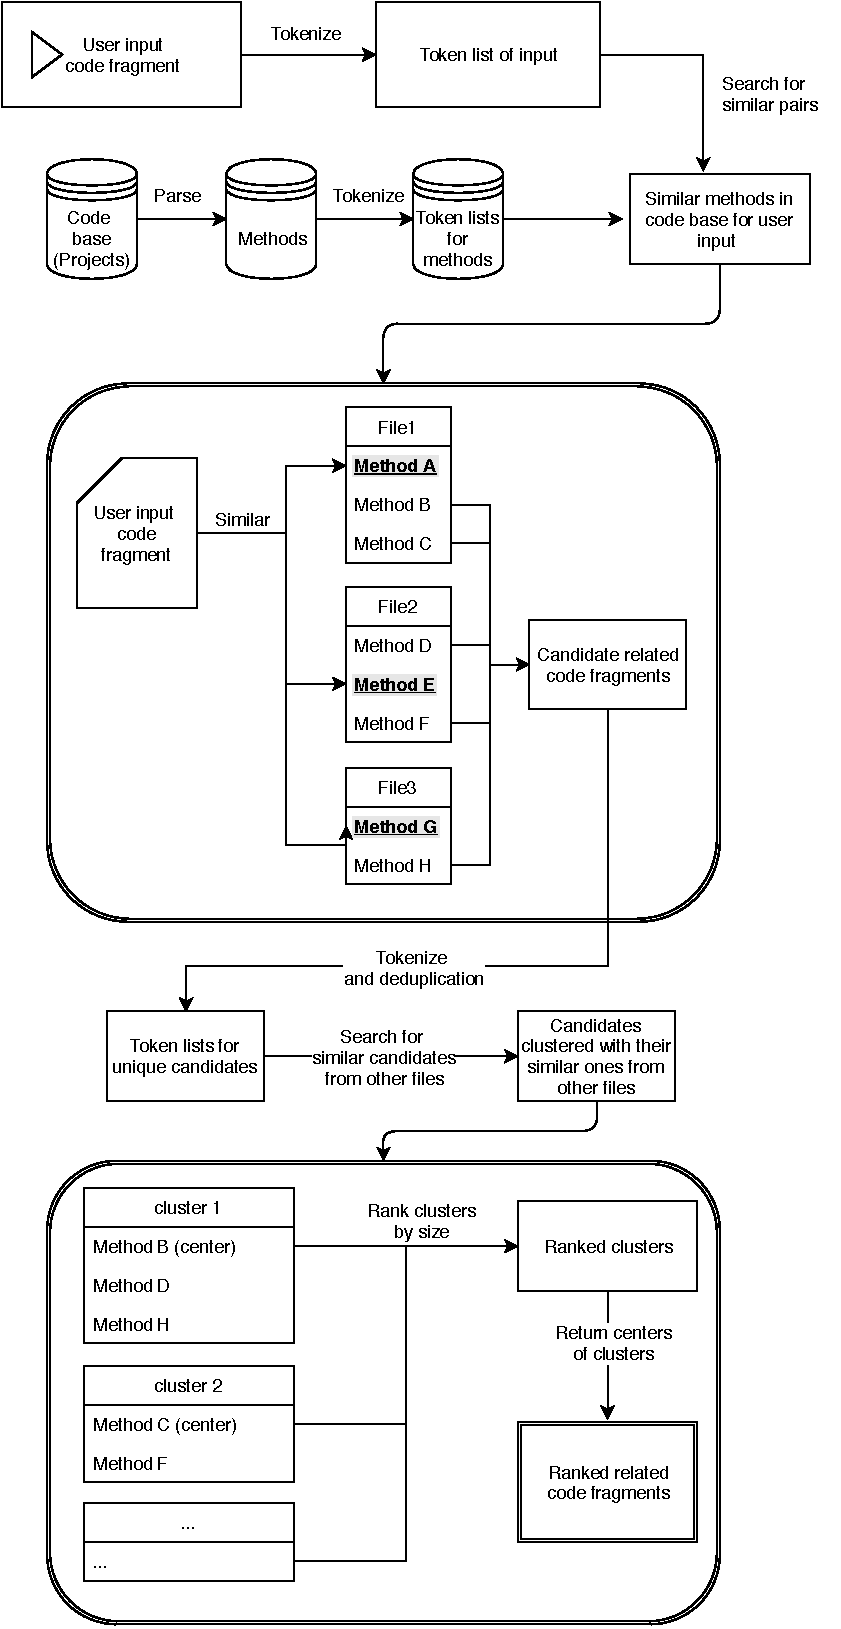
\includegraphics[width=\linewidth]{figures/pipeline.pdf}
	\caption{The pipeline of CodeAid}
	\label{fig:pipeline}
\end{figure}

\subsection{Retrieve similar methods}
\subsubsection{Parse a code corpus}
We focus on method-level code fragments written in Java in this work. We parse all Java source files to abstract syntax trees (ASTs) and traverse the ASTs to extract all defined methods.

\subsubsection{Tokenization}
Tokenization is the process of transforming source code into a bag of words. Tokenization starts from removing comments, spaces, tabs and other special characters. Then it identifies distinct tokens and count their frequencies. For each method, the result of tokenization is formated as a list of tuples such as {\ttt (token, freq)}, where the first element is a token in the method and the second element refers to the token occurrence in the method.
%\begin{lstlisting}
%[(token1, freq1), (token2, freq2), 
%(token3, freq3), ...)]
%\end{lstlisting}
We tokenize both the input code fragment and all methods in the code corpus, in preparation for the next step of finding similar pairs.

\subsubsection{Search for similar methods}
For the input code fragment, we retrieve its similar counterparts from the code corpus using a token-based clone detection technique called SoucererCC~\cite{sajnani2016sourcerercc}. By evaluating the scalability, execution time, recall and precision of SourcererCC, and comparing it to publicly available and state-of-the-art tools, SourcererCC has been shown to have both high recall and precision, and is able to scale to a large repository using a standard workstation. All of the above make SourcererCC a good candidate for building our code recommendation engine. Given a similarity threshold, SoucererCC takes three steps to detect clones. First, it tokenizes a code snippet to a set of tokens. This tokenization step removes comments, whitespaces, and special characters and also counts the frequency of individual tokens. Second, SoucererCC creates a partial index of each snippet by selecting and indexing a subset of tokens based on heuristics, and builds an inverted index mapping between tokens and code snippets. Finally, SoucererCC iterates through all snippets and finds candidate clones of each snippet by querying the inverted index mapping. After retrieving the candidates, SoucererCC uses another heuristic which exploits ordering of the tokens in a snippet to verify the candidates and locate the clones. We use 70\% similarity threshold, because it yields the best precision and recall on multiple clone benchmarks~\cite{sajnani2016sourcerercc}. 

\subsection{Identify co-occurred code fragments}
Given those similar code fragments identified in the previous step, we trace back to the files that contain these similar counterparts and identify co-occurring methods in the same file as a potentially related code fragment. \todo{This step reads a little thin. Having a formal definition here may look better.}  For example, in Figure \ref{fig:pipeline}, the user-selected example is similar to Method A in File 1, Method E in File 2, and Method G in File 3. File 1 also contains Method B and C, File 2 contains Method D and F, and Method H is File 3. Method B, C, D, F, and H will be our candidate for related code fragments, since they co-occur in the same file with similar methods to the user input. 

\subsection{Clustering and Ranking}
%\subsubsection{Search similar methods for each candidate}
\subsubsection{Clustering candidate related code fragments}
We further cluster those candidate related methods identified in the previous step based on their token similarity, in order to detect common co-occurring code fragments. Given each candidate related method, we retrieve its token list again and computes its similarity to other candidates. For example, Method B in File 1 is similar to Method D in File 2 and Method H in File 3, Method C in File 1 is similar to Method F in File 2. \todo{explain this example as a clustering process instead of searching.} \todo{You may also want to redraw the pipeline to reflect the clustering process.}

\subsubsection{Rank by number of similar methods}
After getting similar methods list for each candidate related method, we rank the candidates by its number of similar counterparts and return the ranked related method to the user.